\documentclass[border=8pt, multi, tikz]{standalone} 
\usepackage{import}
\subimport{../../layers/}{init}
\usetikzlibrary{positioning, calc, 3d}

% Color definitions
\def\ConvColor{rgb:yellow,5;red,2.5;white,5}
\def\ConvReluColor{rgb:yellow,5;red,5;white,5}
\def\PoolColor{rgb:red,1;black,0.3}
\def\FcColor{rgb:blue,5;red,2.5;white,5}
\def\SoftmaxColor{rgb:magenta,5;black,7}   

% Arrow styles
\tikzstyle{connection}=[ultra thick, every node/.style={sloped, allow upside down}, draw=black, opacity=0.7]
\tikzstyle{skipconnection}=[ultra thick, dashed, draw=blue, opacity=0.7]

\begin{document}
\begin{tikzpicture}

% Input image
\node[canvas is zy plane at x=0] (input) at (-5,0,0) 
{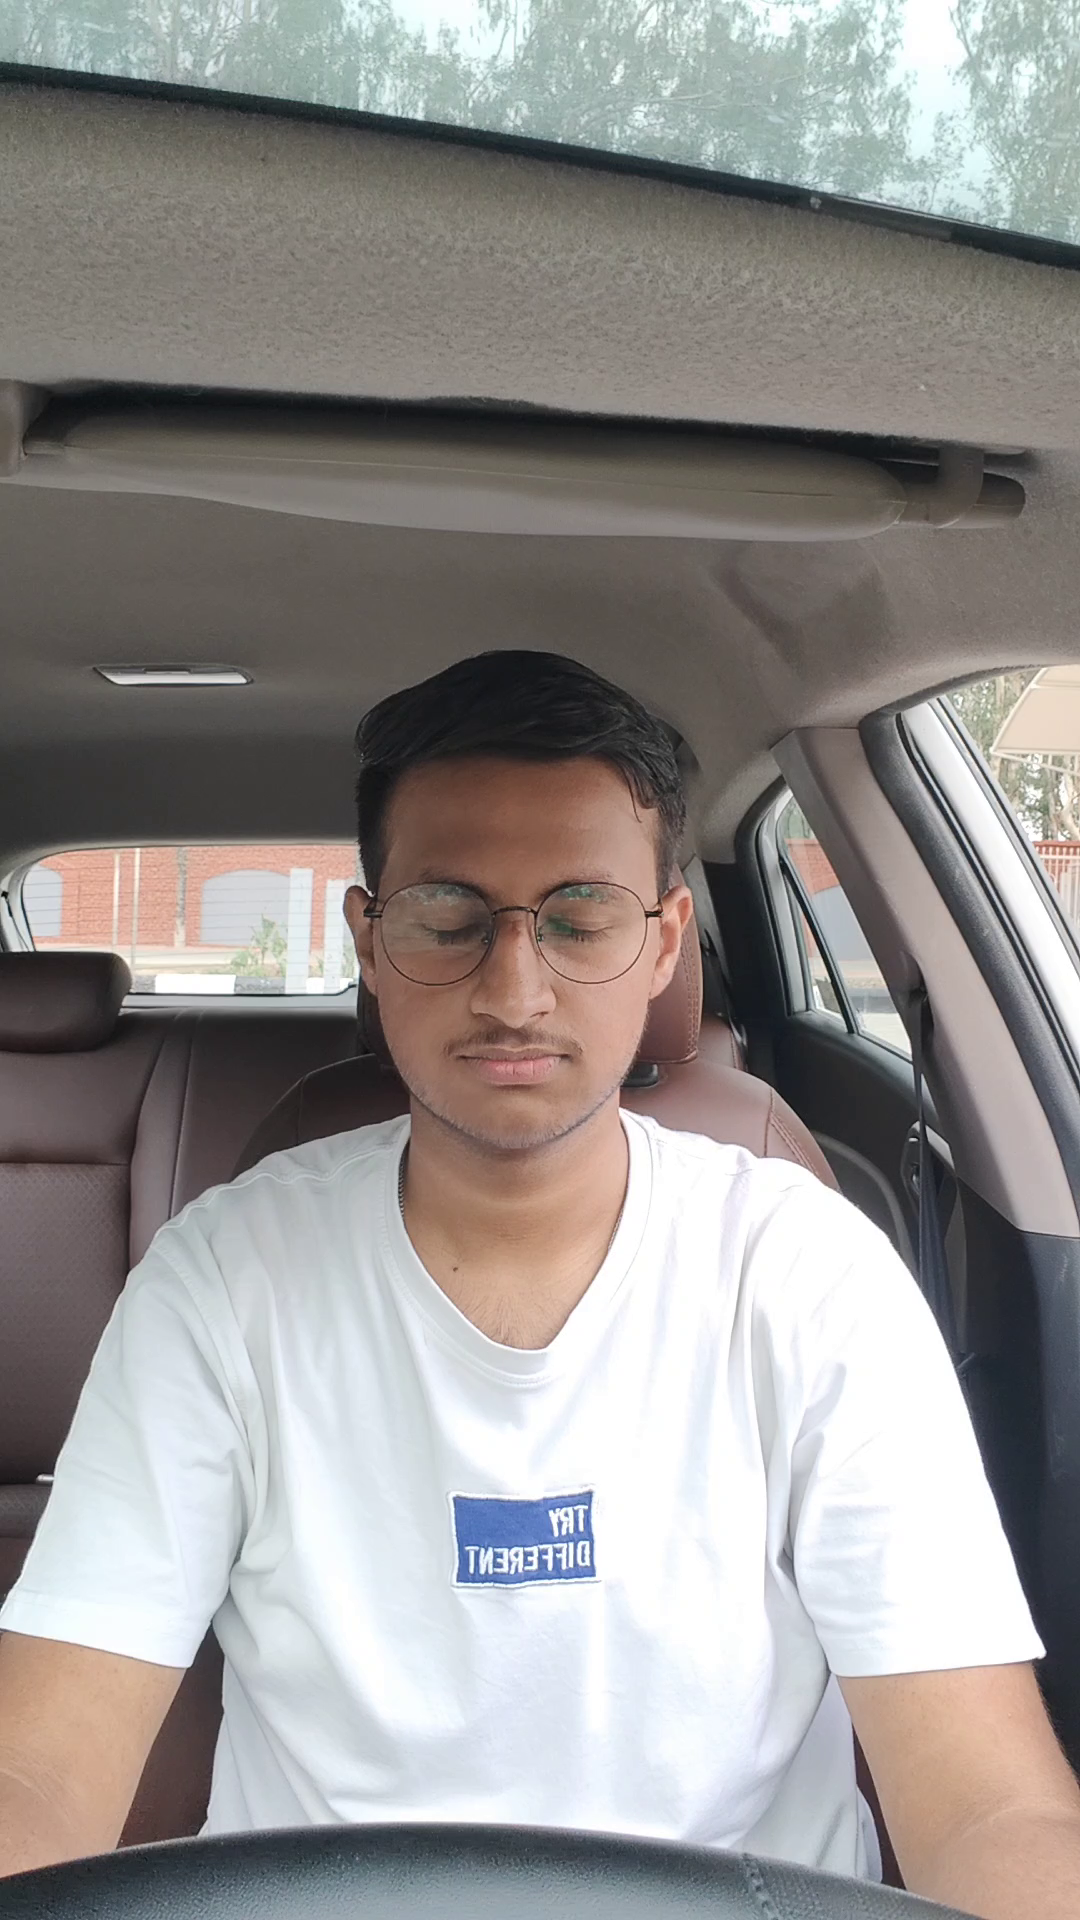
\includegraphics[draft=false, width=6cm,height=6cm]{drowsy.png}};

% Initial Convolution Layer
\pic[shift={(2,0,0)}] at (input.east) 
    {RightBandedBox={
        name=conv1,
        caption=Conv1,
        xlabel={{64,64}},
        zlabel=224,
        fill=\ConvColor,
        bandfill=\ConvReluColor,
        height=40,
        width={2,2},
        depth=40
        }
    };
\draw [connection] (input.east) -- node {\midarrow} (conv1-west);

% Define the number of layers in each Dense Block (DenseNet-121)
\def\nlayersA{6}
\def\nlayersB{12}
\def\nlayersC{24}
\def\nlayersD{16}

% Dense Block 1
\pic[shift={(1,0,0)}] at (conv1-east) 
    {RightBandedBox={
        name=db1,
        caption=Dense Block 1 (\nlayersA Layers),
        xlabel={{128,128}},
        zlabel=112,
        fill=\ConvColor,
        bandfill=\ConvReluColor,
        height=32,
        width={3.5,3.5},
        depth=32
        }
    };
\draw [connection] (conv1-east) -- node {\midarrow} (db1-west);

% Transition Layer 1
\pic[shift={(1,0,0)}] at (db1-east) 
    {Box={
        name=pool1,
        caption=Transition 1,
        fill=\PoolColor,
        height=24,
        width=1,
        depth=24
        }
    };
\draw [connection] (db1-east) -- node {\midarrow} (pool1-west);

% Dense Block 2
\pic[shift={(1,0,0)}] at (pool1-east) 
    {RightBandedBox={
        name=db2,
        caption=Dense Block 2 (\nlayersB Layers),
        xlabel={{256,256}},
        zlabel=56,
        fill=\ConvColor,
        bandfill=\ConvReluColor,
        height=25,
        width={4.5,4.5},
        depth=25
        }
    };
\draw [connection] (pool1-east) -- node {\midarrow} (db2-west);
\draw [skipconnection] (conv1-east) -- (db2-west);

% Transition Layer 2
\pic[shift={(1,0,0)}] at (db2-east) 
    {Box={
        name=pool2,
        caption=Transition 2,
        fill=\PoolColor,
        height=19,
        width=1,
        depth=19
        }
    };
\draw [connection] (db2-east) -- node {\midarrow} (pool2-west);

% Dense Block 3
\pic[shift={(1,0,0)}] at (pool2-east) 
    {RightBandedBox={
        name=db3,
        caption=Dense Block 3 (\nlayersC Layers),
        xlabel={{512,512}},
        zlabel=28,
        fill=\ConvColor,
        bandfill=\ConvReluColor,
        height=16,
        width={5.5,5.5},
        depth=16
        }
    };
\draw [connection] (pool2-east) -- node {\midarrow} (db3-west);
\draw [skipconnection] (db1-west) -- (db3-west);

% Transition Layer 3
\pic[shift={(1,0,0)}] at (db3-east) 
    {Box={
        name=pool3,
        caption=Transition 3,
        fill=\PoolColor,
        height=12,
        width=1,
        depth=12
        }
    };
\draw [connection] (db3-east) -- node {\midarrow} (pool3-west);

% Dense Block 4
\pic[shift={(1,0,0)}] at (pool3-east) 
    {RightBandedBox={
        name=db4,
        caption=Dense Block 4 (\nlayersD Layers),
        xlabel={{1024,1024}},
        zlabel=14,
        fill=\ConvColor,
        bandfill=\ConvReluColor,
        height=10,
        width={6.5,6.5},
        depth=10
        }
    };
\draw [connection] (pool3-east) -- node {\midarrow} (db4-west);
\draw [skipconnection] (db2-west) -- (db4-west);

% Flatten Layer
\pic[shift={(2,0,0)}] at (db4-east) 
    {Box={
        name=flatten,
        caption=Flatten,
        zlabel=7,
        fill=\SoftmaxColor,
        height=1,
        width=1,
        depth=40
        }
    };
\draw [connection] (db4-east) -- node {\midarrow} (flatten-west);

% Fully Connected Layers
\pic[shift={(1,0,0)}] at (flatten-east) 
    {Box={
        name=fc1,
        caption=Dense 512,
        zlabel=1,
        fill=\SoftmaxColor,
        height=1,
        width=1,
        depth=30
        }
    };
\draw [connection] (flatten-east) -- node {\midarrow} (fc1-west);

\pic[shift={(1,0,0)}] at (fc1-east) 
    {Box={
        name=fc2,
        caption=Dense Softmax,
        zlabel=1,
        fill=\SoftmaxColor,
        height=1,
        width=1,
        depth=20
        }
    };
\draw [connection] (fc1-east) -- node {\midarrow} (fc2-west);

% Output Layer
\pic[shift={(1,0,0)}] at (fc2-east) 
    {Box={
        name=softmax,
        caption=Output,
        xlabel={{" ","dummy"}},
        zlabel=5,
        fill=\SoftmaxColor,
        opacity=0.8,
        height=3,
        width=1.5,
        depth=25
        }
    };
\draw [connection] (fc2-east) -- node {\midarrow} (softmax-west);

\end{tikzpicture}
\end{document}
